\subsection{先行研究による知見}
\subsubsection{神経回路シミュレーションの手動での最適化}
\label{sec:section1-1-1}
神経回路シミュレーションを手動で最適化する取り組みは当研究室でも行われてきた.
宮本\cite{miyamoto-master}\cite{miyamoto-master-eng}らの研究では, 神経回路シミュレーションを行うためのソフトウェアであるNEURONの上で
イオンチャネルモデルの一つであるHodgkin-Huxley型モデルを対象として最適化を行った.\\
 NEURONの詳細については後述(\ref{subsec:neuron})するが, NEURONではMODファイルと呼ばれる神経細胞モデルを記述するファイルが
C言語ファイルに変換され実行形式が生成される. しかしながらここで生成されるC言語ファイルには無駄が多いため, 生成されたファイルを
より計算機やモデルの特性にあった形に手動で修正することが可能である.\\
 宮本\cite{miyamoto-master}\cite{miyamoto-master-eng}らの研究において対象とした計算機はスーパーコンピュータ京であり, 京上で十分な性能を発揮するため以下にあげるような最適化を行った.\\
\vspace{-0.5cm}
\begin{enumerate}
\item 常微分方程式の変数を配列化することによるSIMD化.
\item 配列構造のくくり出し.
\item OpenMPとMPIを用いてのハイブリッド並列化.
\item ノード配置の最適化.
\end{enumerate}
 この中で, 本研究では1-3を対象としてNEURON上でのシミュレーションコードの自動最適化を目指す.\\


\subsubsection{神経回路シミュレーションのベンチマークモデル}
\label{subsec:bench-model}
\ref{sec:section1-1-1}項において行った最適化の効果を定量的に評価するため,
宮本\cite{miyamoto-master}\cite{miyamoto-master-eng}らは神経回路シミュレーションのベンチマークモデルを作成し,
次に示す3種類のネットワークを構築することで最適化の効果を測っている.\\
\begin{enumerate}
\item リングネットワーク
\item ランダムネットワーク
\item Watts and Strogatzネットワーク
\end{enumerate}

以下に, 各ネットワークの概要と疑似コードを示す. また, 疑似コード内での定数と関数については
\begin{itemize}
\item NCELL : 細胞数
\item NSYNAPSE : 細胞1つあたりのシナプス数
\item RND : 1以上かつ細胞数より少ない整数の乱数
\item makeSynapse(X, Y) : シナプス前末端を細胞X, シナプス後末端を細胞Yに作成し接続する
\end{itemize}
とし, 細胞内でのシナプスの位置はランダムとした.\\
\clearpage
\begin{figure}[h]
% h:here, t:top, b:bottom, p:page
 \begin{center}
%    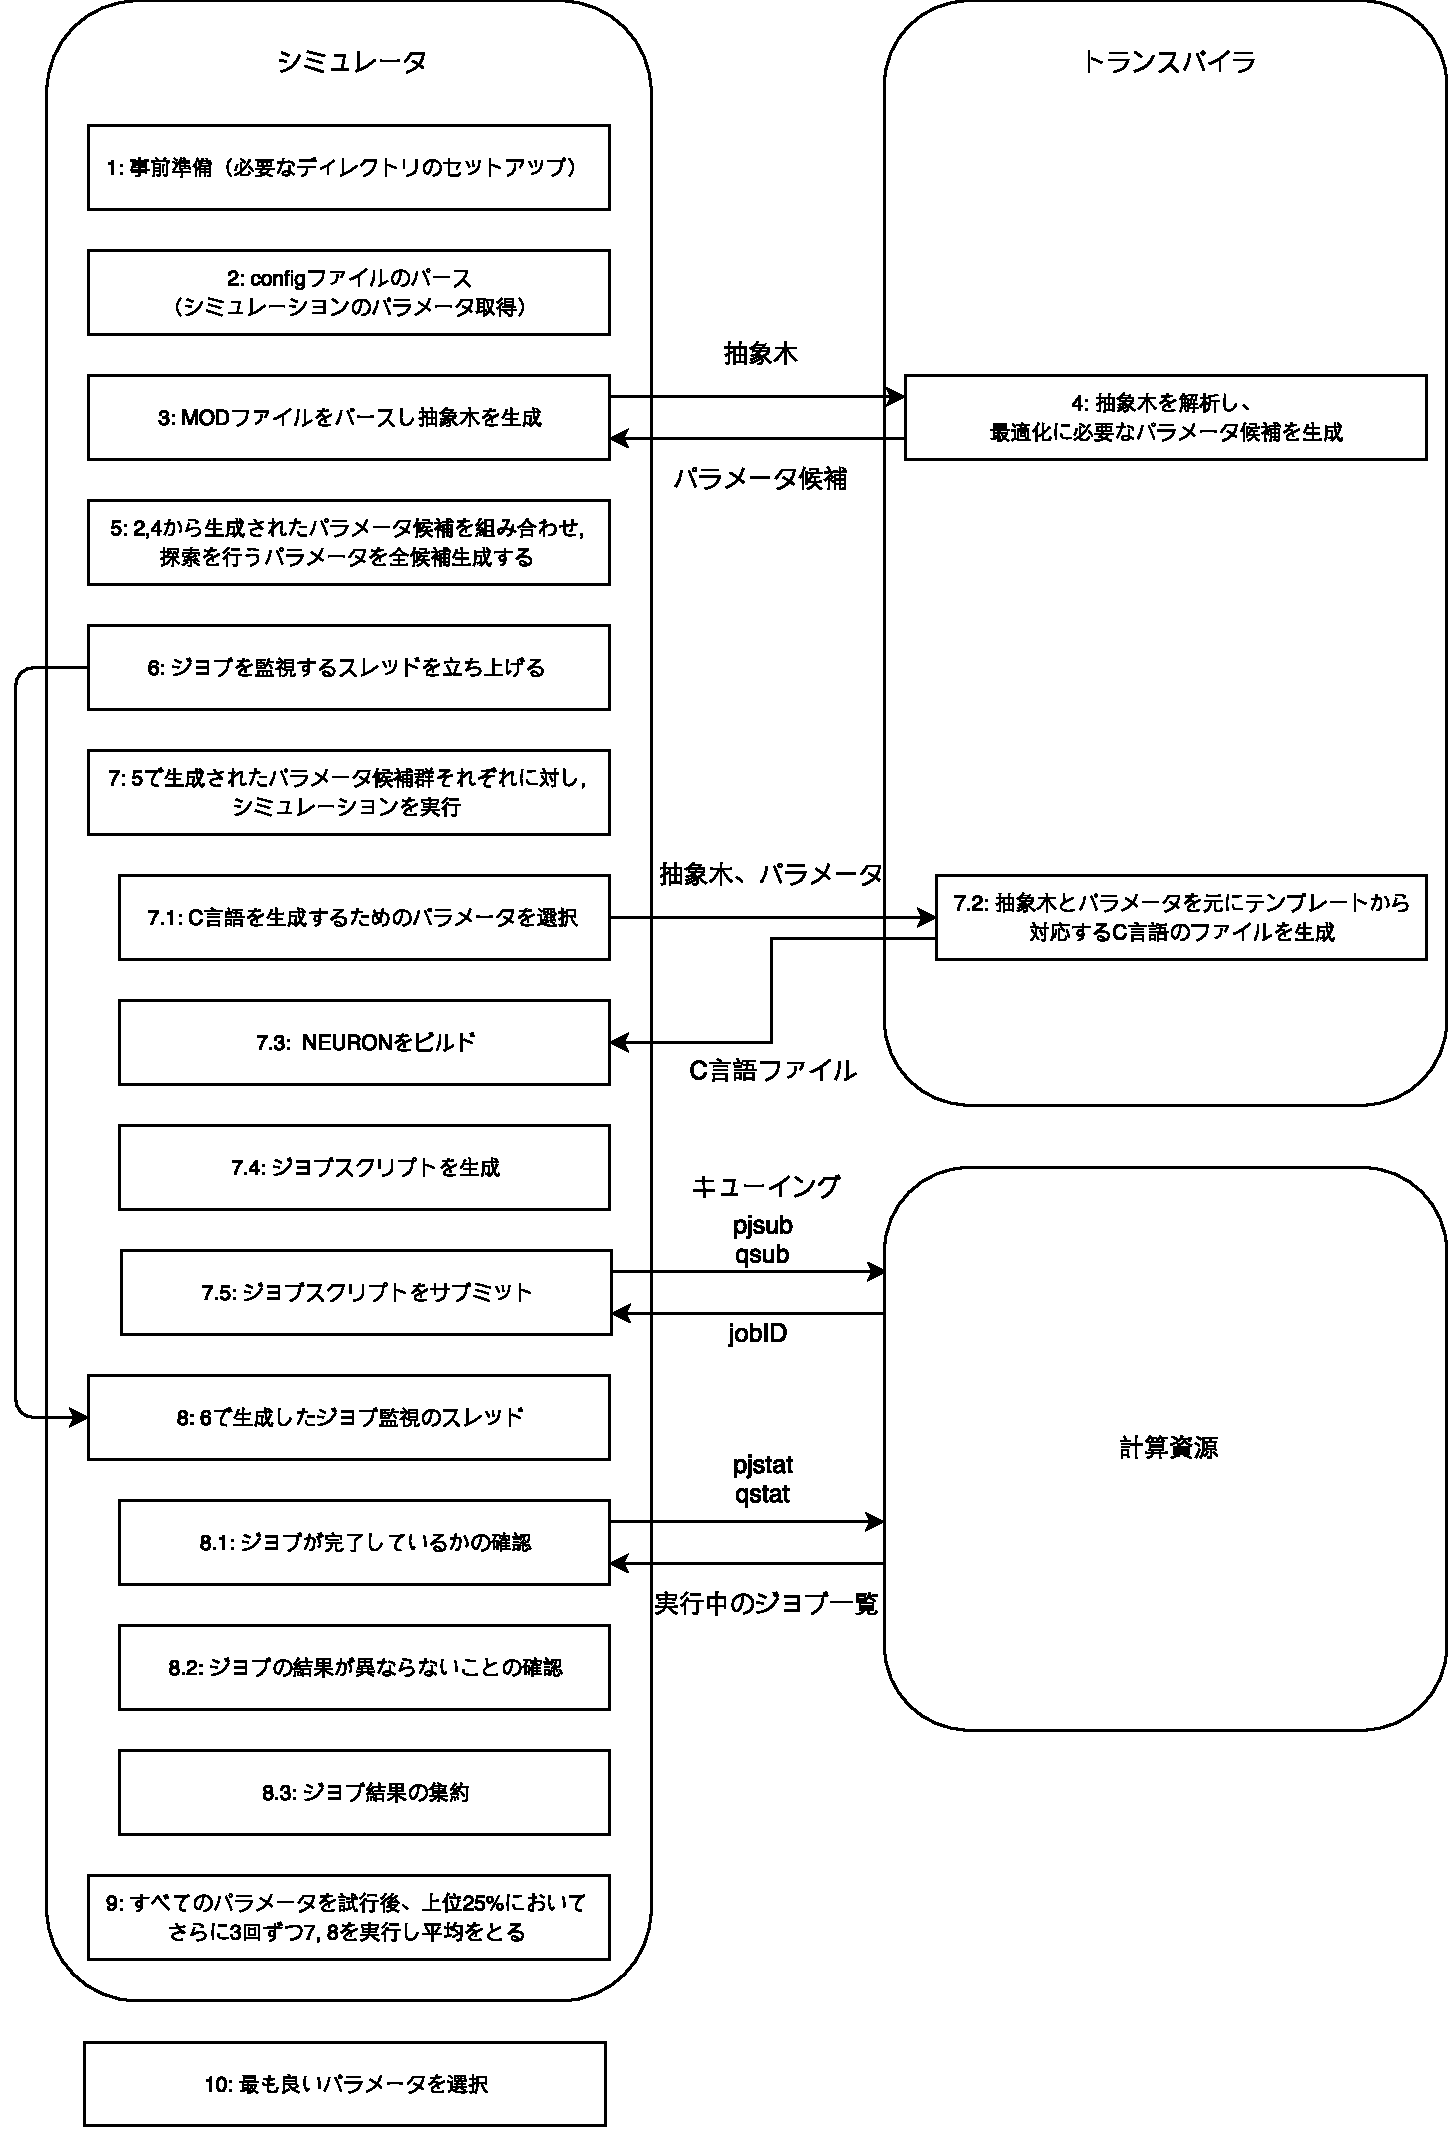
\includegraphics[width=18.0cm]{./images/Genie.pdf}
    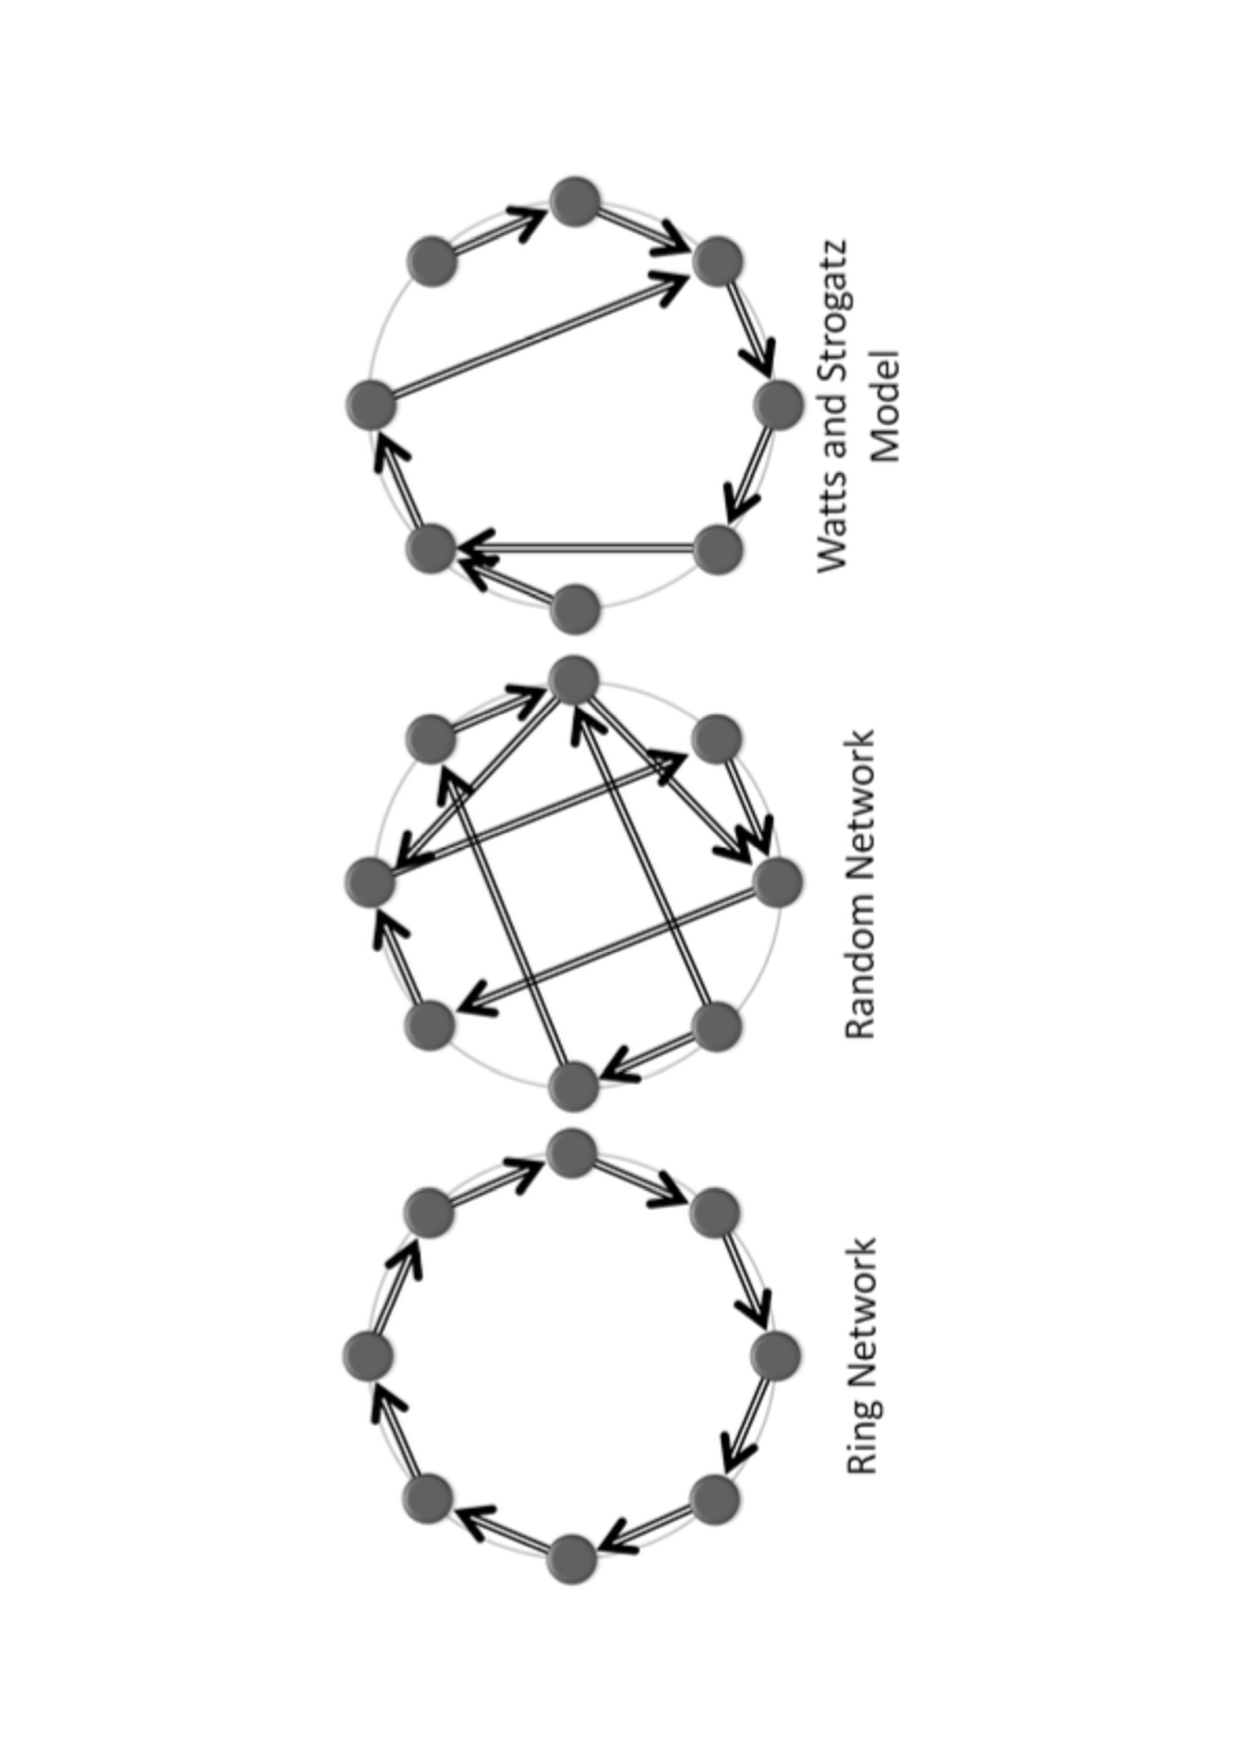
\includegraphics[width=10cm, angle=-90]{./images/bench.pdf}
    \caption[ベンチマークに用いたネットワーク]{ベンチマークに用いたネットワーク (宮本 大輔, カイコガ全脳シミュレーションに向けた三次元モデル及び大規模計算環境の構築, 修士論文, 東京大学, 2014\cite{miyamoto-master})より引用}
    \label{fig:bench-network}
 \end{center}
\end{figure}~\\

\paragraph{リングネットワーク}~\\
 隣り合った細胞同士でシナプスを作成する.\\
\begin{table}[htb]
  \begin{center}
\title{リングネットワークの作成}
{\footnotesize
\begin{framed}
\begin{verbatim}
for (int i=0; i<NCELL; i++) {
    for (int j=0; j<NSYNAPSE; j++) {
        makeSynapse(i, i+1 mod NCELL);
    }
}
\end{verbatim}
\end{framed}
}
\end{center}
\end{table}
\vspace{5cm}
\paragraph{ランダムネットワーク}~\\
 シナプスの前末端はリングネットワークと同様で, シナプスの後末端の位置がランダムなネットワーク.
\begin{table}[htb]
  \begin{center}
\title {ランダムネットワークの作成}
{\footnotesize
\begin{framed}
\begin{verbatim}
for (int i=0; i<NCELL; i++) {
    for (int j=0; j<NSYNAPSE; j++) {
        makeSynapse(i, (i+RND) mod NCELL);
    }
}
\end{verbatim}
\end{framed}
}
\end{center}
\end{table}
\paragraph{Watts and Strogatzネットワーク}~\\
 実際の神経回路ネットワークは, リングでも完全なランダムでもないと考えられる.
そこで宮本\cite{miyamoto-master}\cite{miyamoto-master-eng}らは, それら2つのネットワークの中間的なネットワークに位置付けられるWatts and Strogatzネットワークについてもベンチマークの対象としている.
Watts and Strogatzネットワークは, リングネットワークを作成した後, 確率 p $<$ 1で後末端をランダムに繋ぎかえるものである.\\
\begin{table}[htb]
  \begin{center}
\title {Watts and Strogatzネットワークの作成}
{\footnotesize
\begin{framed}
\begin{verbatim}
P = NSYNAPSE * p;
for (int i=0; i<NCELL; i++) {
    for (int j=0; j<P; j++) {
        makeSynapse(i, (i+RND) mod NCELL);
    }
    for (int j=P; j<NSYNAPSE; j++) {
        makeSynapse(i, i+1 mod NCELL);
    }
}
\end{verbatim}
\end{framed}
}
\end{center}
\end{table}
\vspace{1cm}
